\documentclass[a4paper,12pt]{article}
%%%%% Pakiety
%% Kodowanie dokumentu
\usepackage{polski}
\usepackage[utf8]{inputenc}
\usepackage[T1]{fontenc}
%% Opcje wyświetlania
\usepackage{times}
\usepackage{anysize}
\usepackage{indentfirst}
\usepackage{hyperref}
%% Reszta narzędzi
\usepackage{xcolor}
\usepackage{graphicx}
\usepackage{listings}

%%%%% Opcje dokumentu
\title{Projekt z mikrokontrolerów - sprawozdanie}
	
\marginsize{2cm}{2cm}{2cm}{2cm}
\sloppy

%%%%% Opcje hiperłącza
\hypersetup{
	colorlinks,
	linkcolor={red!50!black},
	citecolor={blue!50!black},
	urlcolor={blue!80!black}
}

%%%%% Do listingu kodu
\lstdefinestyle{customc}{
%%% Kształt całości
	belowcaptionskip=1\baselineskip,
	breaklines=true,
	frame=L,
	xleftmargin=\parindent,
	language=C,
	showstringspaces=false,
%%% Numery linii kodu
	numberfirstline=true,
	numbers=left,
	stepnumber=5,    
	firstnumber=1,
%%% Formatowanie kolorów i czcionki
	basicstyle=\footnotesize\ttfamily,
	morekeywords = {boolean, byte, inline},
	keywordstyle=\bfseries\color{green!40!black},
	commentstyle=\itshape\color{purple!40!black},
	identifierstyle=\color{blue},
	stringstyle=\color{orange},
%%% Polskie znaki
	inputencoding=utf8x, 
	extendedchars=\true,
	literate={ą}{{\k{a}}}1
				{Ą}{{\k{A}}}1
				{ę}{{\k{e}}}1
				{Ę}{{\k{E}}}1
				{ó}{{\'o}}1
				{Ó}{{\'O}}1
				{ś}{{\'s}}1
				{Ś}{{\'S}}1
				{ł}{{\l{}}}1
				{Ł}{{\L{}}}1
				{ż}{{\.z}}1
				{Ż}{{\.Z}}1
				{ź}{{\'z}}1
				{Ź}{{\'Z}}1
				{ć}{{\'c}}1
				{Ć}{{\'C}}1
				{ń}{{\'n}}1
				{Ń}{{\'N}}1
}

\lstset{style=customc}

%%%%%%%%%%%%%%%
\begin{document}

\maketitle

%%%%%%%%%%%%%%%
\section{Informacje ogólne}
\par 1. Temat: Łamanie kodu 
\par 2. Numer grupy: 1b
\par 3. Sklad osobowy: Sebastian Domarecki, Yurii Piets
\par 4. Kierunek: informatyka
\par 5. Rok studiów: II
\par 6. Rok akademicki: 2016-2017

%%%%%%%%%%%%%%%
\section{Opis działania}
%%%
\subsection{Schemat połączenia}

\begin{figure}[!ht]
	
	\centering
	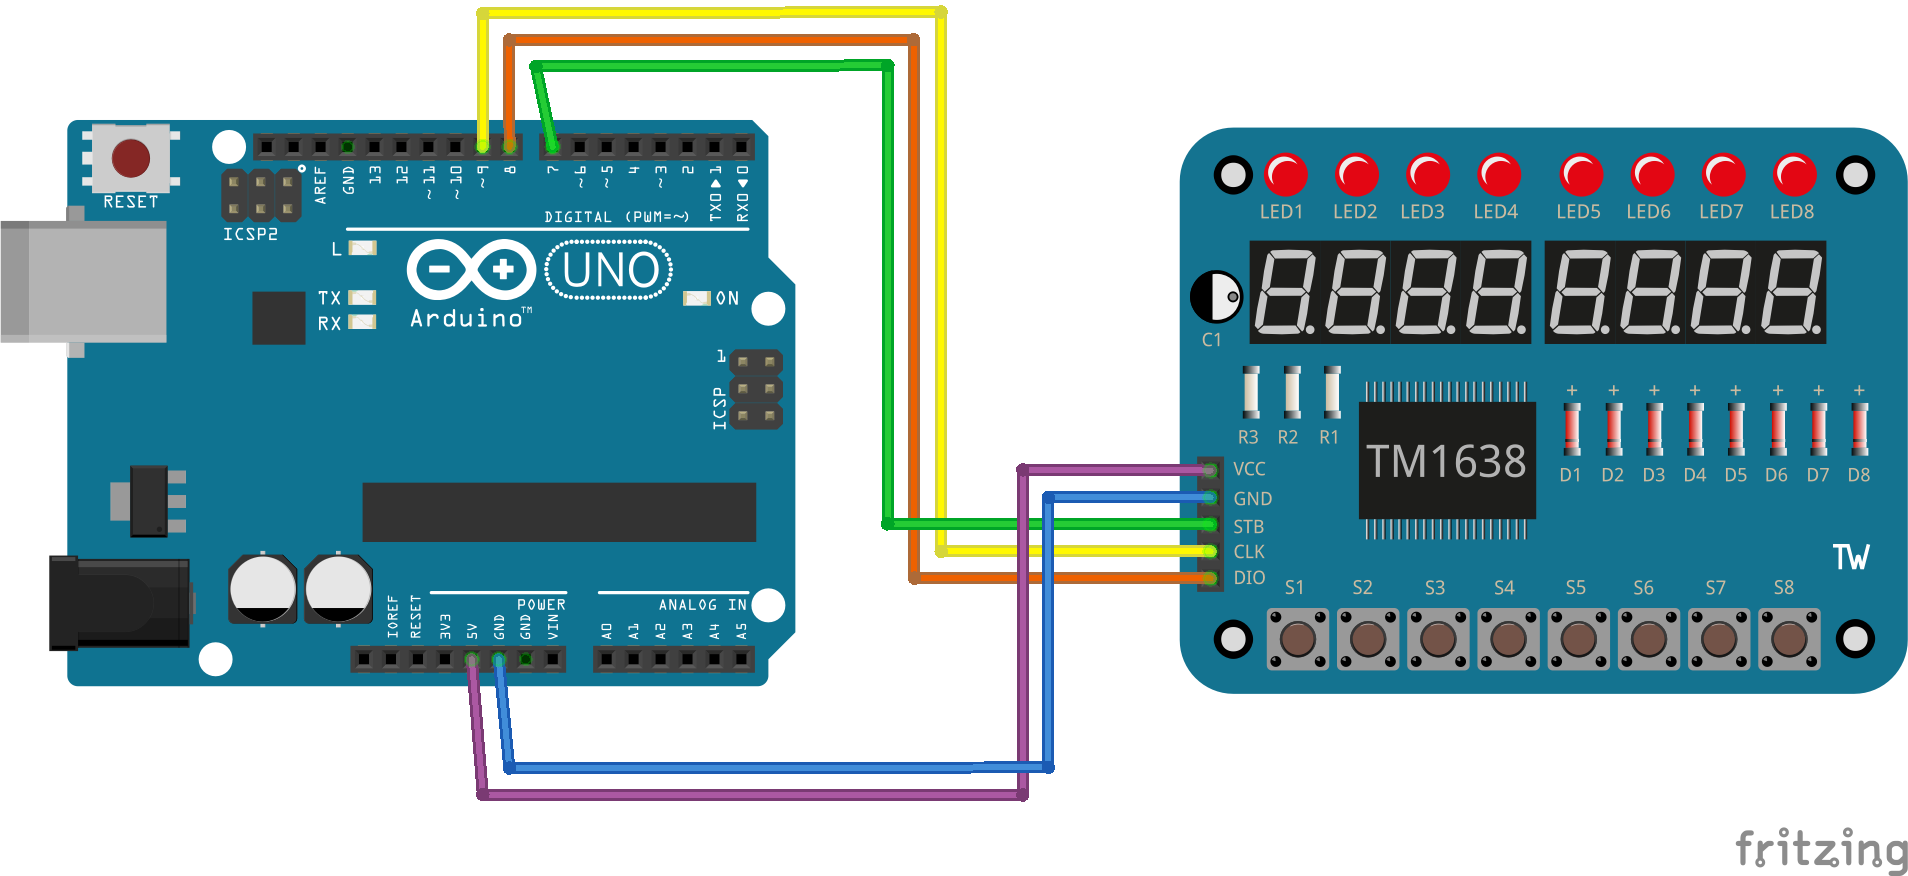
\includegraphics[scale=0.5]{Mikro_bb.png}
	\qquad
	\begin{tabular}[b]{cc}\hline
		TM1638 & Arduino \\ \hline
		VCC & 5V \\
		GND & GND \\
		STB & Digital 7 \\
		CLK & Digital 9 \\
		DIO & Digital 8 \\ \hline
	\end{tabular}
	\label{fig:schemat}
\end{figure}
%%%
\subsection{Opis algorytmu}
Schemat działania algorytmu opiera się w głównej mierze na zredukowanej zewnętrznej bibliotece TM1638.h udostępnianej na \href{https://github.com/rjbatista/tm1638-library}{Githubie}. \\
Program po inicjalizacji ekranu stringiem "00000000", następnie aż do zakończenia łamania kodu znajduje się w pętli iterowanej po numerze dekodowanej cyfry.\\
Wewnątrz niej kolejna pętla for TIMES razy zmienia wyświetlane wartości niezdekodowanych cyfr na wygenerowane przypadowe dozwolone.\\
Za każdą iteracją drugiej pętli sprawdzane jest czy został wciśnięty przycisk, bądź wprowadzona komenda przez port szeregowy.\\
Po jej opuszczeniu włączany jest kolejny led oraz kopiowana wartość zdekodowanej cyfry z CODE do tablicy display do wyświetlenia.
%%%
\subsection{Elementy programu}

\subsubsection{Zmienne}
\par CODE,TIMES,DISP - zgodnie z wytycznymi.
\par module - obiekt klasy TM1638 udostępniający prosty interfejs do obsługi płytki
\par state - zmienna typu wyliczeniowego wyświetlająca stan programu - dostępne IN\_PROGRESS, WAITING, FINISHED, RESET
\subsubsection{Stałe}
\par strobe,clock,data - piny Arduino łączące się z płytką TM1638
\par DISPLAY\_SIZE - wielkość wyświetlacza płytki
\par allowed\_chars - tablica zawierająca dozwolone do wyświetlenia znaki, wszystkie inne są odrzucone
\subsubsection{Funkcje}
\par void handleClick(states *) - obsługa przycisków
\par void readInput(states *) - obsługa poleceń z łącza szeregowego
\par boolean initCode() , initTimes(), initDisp() - wywoływane przy readInput dla pierwszego przesłanego znaku odpowiednio C, N lub D, sczytują z łącza szeregowego nową wartość parametru pracy programu
\par boolean isAllowed(char) - pomocnicza funkcja sprawdzająca czy argument jest dozwolonym znakiem
\par inline void waitTillRelease() - pomocnicza funkcja czekająca na zwolnienie wszystkich przycisków

%%%
\subsection{Biblioteki}
Autorsko zredukowana wersja TM1638.h udostępniana na licencji GNU GPL v3 przez Ricardo Batista.\\
Link: \href{https://github.com/rjbatista/tm1638-library}{https://github.com/rjbatista/tm1638-library}

%%%%%%%%%%%%%%%
\section{Listing kodu}
\lstinputlisting{src_DOMA_PIETS.ino}

%%%%%%%%%%%%%%%
\end{document}
